\subsection{Describe interaction of atoms with light by using the Einstein coefficients. Establish relationships between these coefficients. Relate the Einstein coefficients to spectroscopic experiments.}


\begin{figure}[!h]
    \centering
    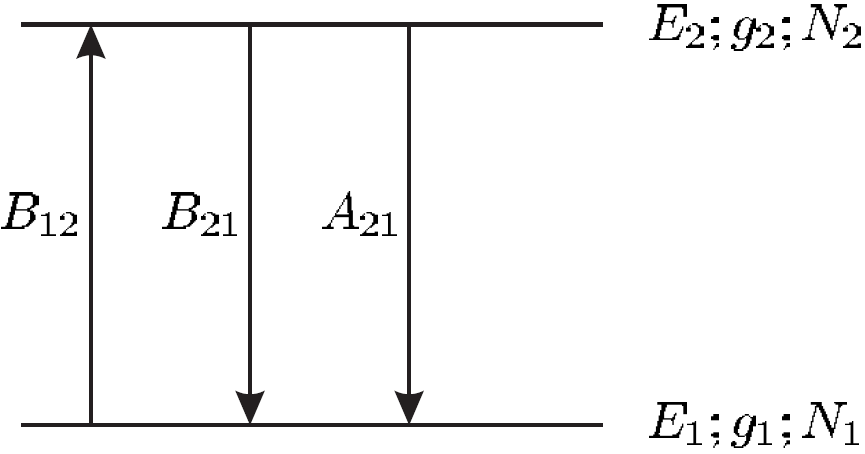
\includegraphics[width=0.5\textwidth]{Q02/images/TwoLevelSystem2.PNG}
    \caption{To-niveausystem med energier $E_1$ og $E_2$, som kan være udarter med $g_1$ og $g_2$, samt har en startpopulation på $N_1$ og $N_2$. Einsteinkoefficienterne $B_{12}$, $B_{21}$ og $A_{21}$ angiver hhv. (stimuleret) absorption, stimuleret emission og spontan emission.}
    \label{fig:Q02_TwoLevelSystem}
\end{figure}

Vi betragter et to-niveausystem med energier $E_1$ og $E_2$. Energiniveauerne har en udartethed (eng. degeneracy) på hhv. $g_1$ og $g_2$, og niveauerne starter med at indeholde hhv. $N_1$ og $N_2$ atomer.


\begin{align}
    \frac{\text{d}N_2}{\text{d}t} &= N_1 B_{12} \rho(\omega_{12}) - N_2 B_{21} \rho(\omega_{12}) - N_2 A_{21}
\end{align}

\begin{align}
    \frac{\text{d}N_1}{\text{d}t} &= - \frac{\text{d}N_2}{\text{d}t}
\end{align}

\begin{align}
    N_2(t) &= N_2(0)\exp{-A_{21}t}
\end{align}


\paragraph{Relation mellem A og B koefficienterne:}

\begin{align}
    \rho(\omega) &= \frac{\hbar\omega}{\pi^2c^3} \dfrac{1}{\exp{\dfrac{\hbar\omega}{k_B T}} - 1}
\end{align}

\begin{align}
    \rho(\omega_{12}) &= \frac{A_{21}}{B_{21}} \dfrac{1}{\dfrac{N_1 B_{12}}{N_2 N_{21}} - 1}
\end{align}

\begin{align}
    \frac{N_2}{g_2} &= \frac{N_1}{g_1}\exp{-\frac{\hbar\omega}{k_B T}}
\end{align}

\begin{align}
    A_{21} & =\frac{\hbar\omega^3}{\pi^2c^3} B_{21}
\end{align}

\begin{align}
    B_{12} &= \frac{g_2}{g_1} B_{12}
\end{align}


\paragraph{Relation af Einsteinkoefficienterne til spektroskopiske eksperimenter:} \ldots




\paragraph{IDEER FRA TØ}

Noter
- S. 11-13
- PP forelæsning 2

To-level atom med energiniveauer E1 og E2. Antal elektroner i hver tilstand, hhv. N1 og N2.
Lys med energitæthed rho(omega) skinner ind på atom => Overgang fra nedre til øvre level med rate proportionalt til rho(omega12), hvor B12 er proportionalitetskonstant. Atomet interagerer meget kun med den del af lyset, som har en frekvens lige omkring omega12 = (E1 - E2)/hbar, hvilket er atomets resonansfrekvens.
Per symmetri formodes det også, at der skabes overgang fra øvre til nedre level med en rate proportional med energidensiteten med proportionalitetskonstant B21.
"This (above) is a process of stimulated emission in which the radiation
at angular frequency $\omega$ causes the atom to emit radiation of the same
frequency."
The symmetry between up and down is broken by the process of spontaneous emission in which an atom falls down to the lower level, even when no external radiation is present. Einstein introduced the coefficient A21 to represent the rate of this process. Thus the rate equations for the populations of the levels, N1 and N2, are eq. (1.25) and (1.26).
Når pho(omega) = 0 og N2 =/= 0 falder populationen i øvre level eksponentielt eq. (1.27), hvor levetiden er 1/A21

Place the atom in a region of black-body radiation: (Equations of page 13)